\documentclass[compress,red]{beamer}
\usepackage[utf8]{inputenc}
\usepackage{ucs}
\usepackage{amsmath}
\usepackage{amsfonts}
\usepackage{amssymb}
\usepackage[russian]{babel}
\usepackage{graphicx}
\usepackage{wrapfig}

\usepackage{tikz}
\usepackage{verbatim}

\usepackage{color}
\usepackage{xcolor}
\usepackage{listings}

\usepackage{caption}

\lstset{
language=sql,
extendedchars=\true,
inputencoding=utf8x,
commentstyle=\itshape,
stringstyle=\bf,
belowcaptionskip=5pt }


\DeclareCaptionFont{white}{\color{white}}
\DeclareCaptionFormat{listing}{\colorbox{gray}{\parbox{\textwidth}{#1#2#3}}}
\captionsetup[lstlisting]{format=listing,labelfont=white,textfont=white}

\usetikzlibrary{calc,trees,positioning,arrows,chains,shapes.geometric,%
    decorations.pathreplacing,decorations.pathmorphing,shapes,%
    matrix,shapes.symbols}

\tikzset{
>=stealth',
  punktchain/.style={
    rectangle, 
    rounded corners, 
    % fill=black!10,
    draw=black, very thick,
    text width=10em, 
    minimum height=3em, 
    text centered, 
    on chain},
  line/.style={draw, thick, <-},
  element/.style={
    tape,
    top color=white,
    bottom color=blue!50!black!60!,
    minimum width=8em,
    draw=blue!40!black!90, very thick,
    text width=10em, 
    minimum height=1.5em, 
    text centered, 
    on chain},
  every join/.style={->, thick,shorten <=1pt},
  decoration={brace},
  tuborg/.style={decorate},
  tubnode/.style={midway, right=2pt},
}

\mode<presentation>

\usetheme{Warsaw}

\definecolor{Red}{rgb}{1,0,0}
\definecolor{Blue}{rgb}{0,0,1}
\definecolor{Green}{rgb}{0,1,0}
\definecolor{magenta}{rgb}{1,0,.6}
\definecolor{lightblue}{rgb}{0,.5,1}
\definecolor{lightpurple}{rgb}{.6,.4,1}
\definecolor{gold}{rgb}{.6,.5,0}
\definecolor{orange}{rgb}{1,0.4,0}
\definecolor{hotpink}{rgb}{1,0,0.5}
\definecolor{newcolor2}{rgb}{.5,.3,.5}
\definecolor{newcolor}{rgb}{0,.3,1}
\definecolor{newcolor3}{rgb}{1,0,.35}
\definecolor{darkgreen1}{rgb}{0, .35, 0}
\definecolor{darkgreen}{rgb}{0, .6, 0}
\definecolor{darkred}{rgb}{.75,0,0}

\xdefinecolor{olive}{cmyk}{0.64,0,0.95,0.4}
\xdefinecolor{purpleish}{cmyk}{0.75,0.75,0,0}

\useoutertheme[subsection=false]{smoothbars}

\title{Язык SQL}
\author{Информатика \\ 10-11 классы}

%\usecolortheme{dolphin}


\begin{document}
%%титульная страница
\maketitle
%% основные моменты

\section{SELECT}

\subsection{Повторим SELECT}
\begin{frame}[fragile]
  \frametitle{Повторим SELECT}
  \centerline{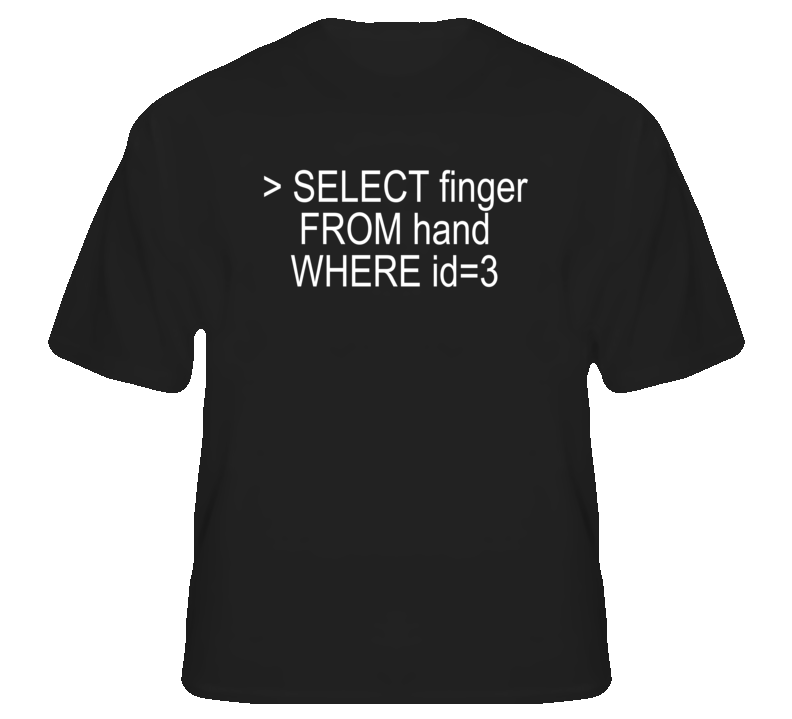
\includegraphics[width=0.7\textwidth]{images/tshirt.png}}
\end{frame}

\subsection{Оператор SELECT}
\begin{frame}[fragile]
  \frametitle{Оператор SELECT}
  \begin{tabular}{|c|c|c|c|c|}
  \hline
  id & first\_name & last\_name & gender & created\_at\\
  \hline
  \end{tabular}
  \begin{itemize}
    \item Вспомним один из простейших запросов:
  \end{itemize}
  \scriptsize{
  \begin{lstlisting}[label=sql1, caption=SELECT]
    SELECT * FROM users
    WHERE (gender = 1)
    ORDER BY created_at DESC
    LIMIT 1
  \end{lstlisting}
  }
\end{frame}

\subsection{Функции}
\begin{frame}[fragile]
  \frametitle{Функции}
  \begin{itemize}[<+->]
    \item Зачастую встаёт задача не просто по выборке каких-либо данных из таблицы, а по их подсчёту.
    \item Пример ``раз'': есть таблица учеников students. Сколько учеников имеет оценку 5?
    \item Пример ``два'': какой максимальный балл набрал ученик за тест?
    \item Пример ``три'': чему равен средний балл по контрольной?
    \item Пример ``четыре'': сколько пользователей банка за последний месяц воспользовались услугами Интернет--банкинга?
    \item Для работы со всем этим и применяются специальные функции. 
  \end{itemize}
\end{frame}

\subsection{Список функций}
\begin{frame}[fragile]
  \frametitle{Функции}
  \begin{tabular}{lp{2cm}p{6cm}}
    \hline
    \hline
    Функция & Аргументы & Описание \\
    \hline
    COUNT(*) & не важно & считает количество записей в выборке \\
    \hline
    MAX(mark) & название столбца & находит максимальное значение в столбце среди выбранных записей \\
    \hline
    MIN(mark) & название столбца & находит минимальное значение в столбце среди выбранных записей \\
    \hline
    SUM(mark) & название столбца & находит сумму значений из столбца mark среди выбранных записей \\
    \hline
    AVG(mark) & название столбца & находит среднее арифметическое значение в столбце среди выбранных записей \\
    \hline
    \hline
  \end{tabular}
\end{frame}

\subsection{COUNT}
\begin{frame}[fragile]
  \frametitle{COUNT}
  \begin{table}
    \begin{tabular}{|c|c|c|c|c|}
      \hline
      id & first\_name & last\_name & gender & created\_at\\
      \hline
    \end{tabular}
    \caption{users}
  \end{table}
  \begin{itemize}
    \item Сколько записей в таблице users?
  \end{itemize}
  \scriptsize{
  \begin{lstlisting}[label=sql2,caption=SELECT COUNT]
    SELECT COUNT(*) FROM users;
  \end{lstlisting}
  \begin{itemize}
    \item Результат: 6
  \end{itemize}
  }
\end{frame}

\subsection{COUNT}
\begin{frame}[fragile]
  \frametitle{COUNT с условием}
  \begin{table}
    \begin{tabular}{|c|c|c|c|c|}
      \hline
      id & first\_name & last\_name & gender & created\_at\\
      \hline
    \end{tabular}
    \caption{users}
  \end{table}
  \begin{itemize}
    \item А сколько мужчин?
  \end{itemize}
  \scriptsize{
  \begin{lstlisting}[label=sql3,caption=SELECT COUNT]
    SELECT COUNT(*) FROM users WHERE gender=1;
  \end{lstlisting}
  \begin{itemize}
    \item Результат: 4
  \end{itemize}
  }
\end{frame}

\subsection{MAX}
\begin{frame}[fragile]
  \frametitle{MAX}
  \begin{table}
    \begin{tabular}{|c|c|c|c|c|}
      \hline
      id & student\_id & gender & mark & created\_at\\
      \hline
    \end{tabular}
    \caption{exam\_results}
  \end{table}
  \begin{itemize}
    \item Какое максимальное (минимальное) количество баллов было набрано на экзамене?
  \end{itemize}
  \scriptsize{
  \begin{lstlisting}[label=sql4,caption=SELECT MAX,MIN]
    SELECT MAX(mark) FROM exam_results;
    SELECT MIN(mark) FROM exam_results;
  \end{lstlisting}
  }
\end{frame}

\subsection{AVG}
\begin{frame}[fragile]
  \frametitle{AVG}
  \begin{table}
    \begin{tabular}{|c|c|c|c|c|}
      \hline
      id & student\_id & gender & mark & created\_at\\
      \hline
    \end{tabular}
    \caption{exam\_results}
  \end{table}
  \begin{itemize}
    \item А каков средний балл?
  \end{itemize}
  \scriptsize{
  \begin{lstlisting}[label=sql5,caption=SELECT AVG]
    SELECT AVG(mark) FROM exam_results;
  \end{lstlisting}
  }
\end{frame}

\section{GROUP BY}
\subsection{GROUP BY}
\begin{frame}[fragile]
  \frametitle{GROUP BY}
  \begin{itemize}
    \item А что, если я хочу узнать, сколько учеников получило оценку 5, сколько 4, и т.п.?
    \item Конечно, можно выполнить ряд последовательных запросов с поиском через WHERE.
    \item Но есть альтернатива! --- \textbf{GROUP BY}.
    \item Оператор GROUP BY группирует результаты по заданному полю.
  \end{itemize}
\end{frame}

\subsection{GROUP BY COUNT}
\begin{frame}[fragile]
  \frametitle{GROUP BY и COUNT}
  \begin{table}
    \begin{tabular}{|c|c|c|c|c|}
      \hline
      id & student\_id & gender & mark & created\_at\\
      \hline
    \end{tabular}
    \caption{exam\_results}
  \end{table}
  \begin{itemize}
    \item Таблица: балл --- количество учеников, его набравших.
  \end{itemize}
  \scriptsize{
  \begin{lstlisting}[label=sql6,caption=GROUP BY]
    SELECT mark, COUNT(*) FROM exam_results
    GROUP BY mark;
  \end{lstlisting}
  }
\end{frame}

\subsection{GROUP BY AVG}
\begin{frame}[fragile]
  \frametitle{GROUP BY и AVG}
  \begin{table}
    \begin{tabular}{|c|c|c|c|c|}
      \hline
      id & student\_id & gender & mark & created\_at\\
      \hline
    \end{tabular}
    \caption{exam\_results}
  \end{table}
  \begin{itemize}
    \item А если ученики писали не один экзамен, а несколько? Как подсчитать средний балл по каждому ученику?
  \end{itemize}
  \scriptsize{
  \begin{lstlisting}[label=sql7,caption=GROUP BY AVG]
    SELECT *, AVG(mark) FROM exam_results
    GROUP BY student_id;
  \end{lstlisting}
  }
\end{frame}

\subsection{GROUP BY HAVING}
\begin{frame}[fragile]
  \frametitle{GROUP BY и HAVING}
  \begin{table}
    \begin{tabular}{|c|c|c|c|c|}
      \hline
      id & student\_id & gender & mark & created\_at\\
      \hline
    \end{tabular}
    \caption{exam\_results}
  \end{table}
  \begin{itemize}
    \item А если я хочу вывести только учеников, у которых средний балл выше 3? При этом отсортировать по убыванию баллов?
  \end{itemize}
  \scriptsize{
  \begin{lstlisting}[label=sql8,caption=GROUP BY HAVING]
    SELECT *, AVG(mark) AS avg_mark FROM exam_results
    GROUP BY student_id
    HAVING avg_mark
    ORDER BY avg_mark DESC;
  \end{lstlisting}
  }
\end{frame}

\section{INSERT, UPDATE, DELETE}
\subsection{INSERT}
\begin{frame}[fragile]
  \frametitle{INSERT}
  \begin{table}
    \begin{tabular}{|c|c|c|c|c|}
      \hline
      id & student\_id & gender & mark & created\_at\\
      \hline
    \end{tabular}
    \caption{exam\_results}
  \end{table}
  \begin{itemize}
    \item Добавляем новую запись в таблицу.
  \end{itemize}
  \scriptsize{
  \begin{lstlisting}[label=sql9,caption=INSERT]
    INSERT INTO exam_results (student_id, gender, mark)
    VALUES (1, 1, 5);
  \end{lstlisting}
  }
\end{frame}

\subsection{UPDATE}
\begin{frame}[fragile]
  \frametitle{UPDATE}
  \begin{table}
    \begin{tabular}{|c|c|c|c|c|}
      \hline
      id & student\_id & gender & mark & created\_at\\
      \hline
    \end{tabular}
    \caption{exam\_results}
  \end{table}
  \begin{itemize}
    \item Изменяем запись в таблицу.
  \end{itemize}
  \scriptsize{
  \begin{lstlisting}[label=sql10,caption=UPDATE]
    UPDATE exam_results SET gender=2, mark=3
    WHERE id = 5;
  \end{lstlisting}
  }
\end{frame}

\subsection{DELETE}
\begin{frame}[fragile]
  \frametitle{DELETE}
  \begin{table}
    \begin{tabular}{|c|c|c|c|c|}
      \hline
      id & student\_id & gender & mark & created\_at\\
      \hline
    \end{tabular}
    \caption{exam\_results}
  \end{table}
  \begin{itemize}
    \item Удаляем.
  \end{itemize}
  \scriptsize{
  \begin{lstlisting}[label=sql11,caption=DELETE]
    DELETE FROM exam_results
    WHERE created_at < "2012-01-01";
  \end{lstlisting}
  }
\end{frame}

\subsection{Тестовая таблица}
\begin{frame}[fragile]
  \frametitle{Тестовая таблица courses}
  \begin{tabular}{|c|c|c|c|c|c|c|}
  \hline
  id & title & desc & type & is\_active & created\_at & updated\_at\\
  \hline
  1 & Ruby & ... & 1 & 1 & 2012-01-01 & 2012-01-01\\
  \hline
  2 & Info & ... & 0 & 0 & 2012-01-02 & 2012-02-01\\
  \hline
  3 & Google & ... & 1 & 0 & 2012-03-25 & 2012-05-28\\
  \hline
  4 & Test & ... & 0 & 1 & 2012-03-25 & 2012-11-13\\
  \hline
  \end{tabular}
\end{frame}

\end{document}